% See SO post for png converstion details - https://tex.stackexchange.com/a/11880
\documentclass[crop]{standalone}
\usepackage{tikz}

\begin{document}
\pagestyle{empty}

\newcommand{\Depth}{3}
\newcommand{\Height}{3}
\newcommand{\Width}{3}

\tikzstyle{line}=[thick]
\begin{tikzpicture}
	\coordinate (O) at (0,0,0);
	\coordinate (A) at (0,\Width,0);
	\coordinate (B) at (0,\Width,\Height);
	\coordinate (C) at (0,0,\Height);
	\coordinate (D) at (\Depth,0,0);
	\coordinate (E) at (\Depth,\Width,0);
	\coordinate (F) at (\Depth,\Width,\Height);
	\coordinate (G) at (\Depth,0,\Height);

	\draw[line] (O) -- (C) -- (G) -- (D) -- cycle;% Bottom Face
	\draw[line] (O) -- (A) -- (E) -- (D) -- cycle;% Back Face
	\draw[line] (O) -- (A) -- (B) -- (C) -- cycle;% Left Face
	\draw[line] (D) -- (E) -- (F) -- (G) -- cycle;% Right Face
	\draw[line] (C) -- (B) -- (F) -- (G) -- cycle;% Front Face
	\draw[line] (A) -- (B) -- (F) -- (E) -- cycle;% Top Face
\end{tikzpicture}

\hspace{1cm}
\tikzstyle{line}=[thick]
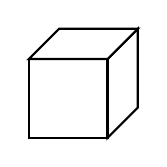
\begin{tikzpicture}
	\coordinate (O) at (0,0,0);
	\coordinate (A) at (0,\Width,0);
	\coordinate (B) at (0,\Width,\Height);
	\coordinate (C) at (0,0,\Height);
	\coordinate (D) at (\Depth,0,0);
	\coordinate (E) at (\Depth,\Width,0);
	\coordinate (F) at (\Depth,\Width,\Height);
	\coordinate (G) at (\Depth,0,\Height);

	% \draw[line] (O) -- (C) -- (G) -- (D) -- cycle;% Bottom Face
	% \draw[line] (O) -- (A) -- (E) -- (D) -- cycle;% Back Face
	% \draw[line] (O) -- (A) -- (B) -- (C) -- cycle;% Left Face
	\draw[fill=white, opacity=1, thick] (D) -- (E) -- (F) -- (G) -- cycle;% Right Face
	\draw[fill=white, opacity=1, thick] (C) -- (B) -- (F) -- (G) -- cycle;% Front Face
	\draw[fill=white, opacity=1, thick] (A) -- (B) -- (F) -- (E) -- cycle;% Top Face
\end{tikzpicture}

\hspace{1cm}
\tikzstyle{line}=[thick]
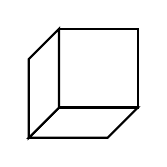
\begin{tikzpicture}
	\coordinate (O) at (0,0,0);
	\coordinate (A) at (0,\Width,0);
	\coordinate (B) at (0,\Width,\Height);
	\coordinate (C) at (0,0,\Height);
	\coordinate (D) at (\Depth,0,0);
	\coordinate (E) at (\Depth,\Width,0);
	\coordinate (F) at (\Depth,\Width,\Height);
	\coordinate (G) at (\Depth,0,\Height);

	\draw[fill=white, opacity=1, thick] (O) -- (C) -- (G) -- (D) -- cycle;% Bottom Face
	\draw[fill=white, opacity=1, thick] (O) -- (A) -- (E) -- (D) -- cycle;% Back Face
	\draw[fill=white, opacity=1, thick] (O) -- (A) -- (B) -- (C) -- cycle;% Left Face
	% \draw[line] (D) -- (E) -- (F) -- (G) -- cycle;% Right Face
	% \draw[line] (C) -- (B) -- (F) -- (G) -- cycle;% Front Face
	% \draw[line] (A) -- (B) -- (F) -- (E) -- cycle;% Top Face
\end{tikzpicture}
\hspace{0.5cm}

\end{document}


